\subsection[Il k-nearest neighbors (k-NN)]{\textit{Il k-nearest neighbors (k-NN)}}
\begin{frame}

	\frametitle{k-nearest neighbors (k-NN)}

%	\begin{block}{}
		L'algoritmo k-nearest neighbors (k-NN) può essere utilizzato sia nella classificazione che nella regressione.
		\newlinedouble
		In entrambi i casi, l'\textbf{input} è costituito dai \textbf{k esempi di addestramento più vicini} nello spazio delle features.
		L'\textbf{output} è diverso a seconda che si stia applicando il k-NN per una classificazione o per una regressione:
		\begin{itemize}
			\item nella regressione k-NN, l'output è \textbf{la media dei valori} dei k vicini più vicini
			\item nella classificazione k-NN, l'output è una \textbf{classe di appartenenza} dei k vicini più vicini
		\end{itemize}

%	\end{block}

\end{frame}


\subsubsection[Regressione k-NN]{\textit{Regressione k-NN}}
\begin{frame}

	\frametitle{Regressione k-NN: prima versione locale}

	\begin{itemize}
		\item vogliamo approssimare $f(x) = \E(Y|X=x)$
		\item sia $c$ una condizione logica, e definiamo
			\[
				\mathbb{I}(c) = \left\{\begin{array}{ll} 1 & \mbox{se $c$ è vera} \\
				0 & \mbox{se $c$ è falsa}
				\end{array} \right.
			\]
		\item Idea:
		\[
			\widehat{f}(x) = \frac{\sum_{i=1}^n y_i \, \mathbb{I}(x_i=x)}{\sum_{i=1}^n \mathbb{I}(x_i=x)} = \mbox{$y_i$ medio, t.c. $x_i=x$}
		\]
		\item questo stimatore è \emph{molto locale}, spesso anche troppo!
	\end{itemize}
	
	\begin{center}
		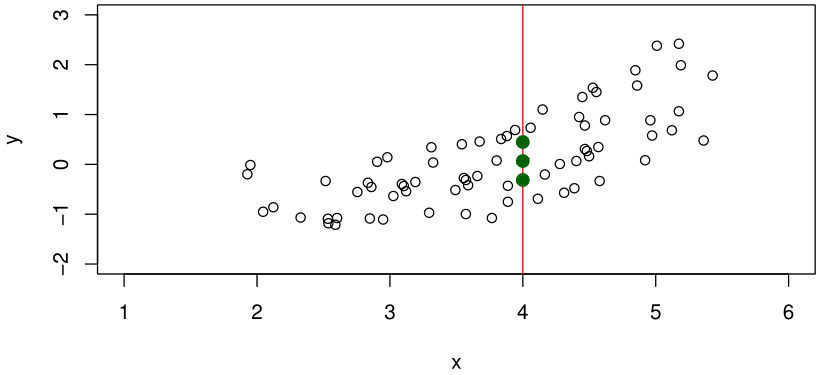
\includegraphics[width=0.6\linewidth]{images/supervised/knn_regression/knn_regression_local.png}
	\end{center}
\end{frame}



\begin{frame}

	\frametitle{Regressione k-NN: seconda versione, intorno $\mathcal{N}(x)$}

	\begin{itemize}
		\item ecco un approccio meno restrittivo: consideriamo un intorno $\mathcal{N}(x)$ di $x$, e usiamo
			\[
				\widehat{f}(x) = \frac{\sum_{i=1}^n y_i\,\mathbb{I}[x\in\mathcal{N}(x)]}{\sum_{i=1}^n \mathbb{I}[x\in\mathcal{N}(x)]} = \mbox{$y_i$ medio, t.c. $x_i\in \mathcal{N}(x)$}
			\]
			\begin{center}
				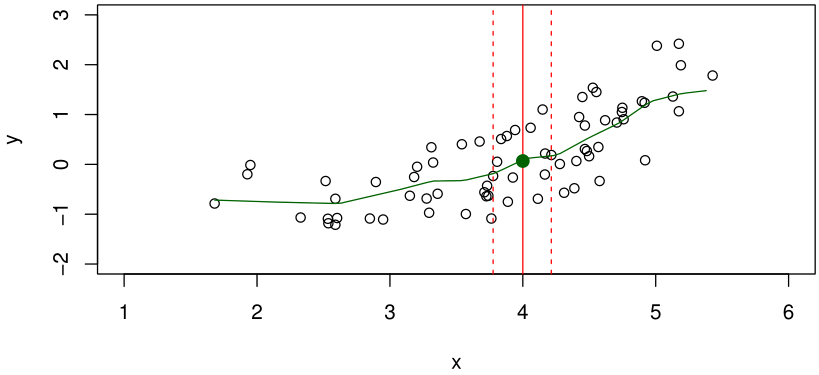
\includegraphics[width=0.75\linewidth]{images/supervised/knn_regression/knn_regression.png}
			\end{center}
		\item questa versione soffre della cosiddetta \textit{maledizione della dimensionalità}
	\end{itemize}
	
\end{frame}


\ifthenelse{\boolean{highschool}}{}{
\begin{frame}

	\frametitle{Regressione k-NN, \textit{maledizione della dimensionalità}}

	\begin{itemize}
		\item per scegliere $\mathcal{N}(x)$ possiamo imporre che contenga una certa percentuale degli $n$ valori di $X$, per esempio $\alpha$\%
		\item k-NN può fornire risultati molto validi per valori di $p=\dim(X)$ piccoli, di solito $p \leq 4$, e $n$ elevato
		\item k-NN è \textbf{inaffidabile per} $\pmb{p}$ \textbf{elevato} a causa della maledizione della dimensionalità
		\item in media, un intorno di ordine $\alpha$\% in uno spazio a molte dimensioni non è locale, e k-NN diventa un metodo estremamente \emph{globale}
		\item per capire perché, consideriamo un esempio molto semplice:
			\begin{itemize}
				\item assumiamo che i $p$ predittori $X_k$ siano tutti IID $\mathcal{U}(0,1)$
				\item approssimativamente, $\alpha$ è il volume dell'ipersfera centrata in $x$ di raggio $r$:
					\[
						\alpha = \frac{\pi^{\frac{p}{2}} r^p}{\Gamma(\frac{p}{2}+1)} \quad \Rightarrow \quad r=\left[\frac{\alpha \Gamma(\frac{p}{2}+1)}{\pi^\frac{p}{2}}\right]^{\frac{1}{p}}
					\]
			\end{itemize}
	\end{itemize}
\end{frame}



\begin{frame}

	\frametitle{Regressione k-NN}

	\begin{center}
		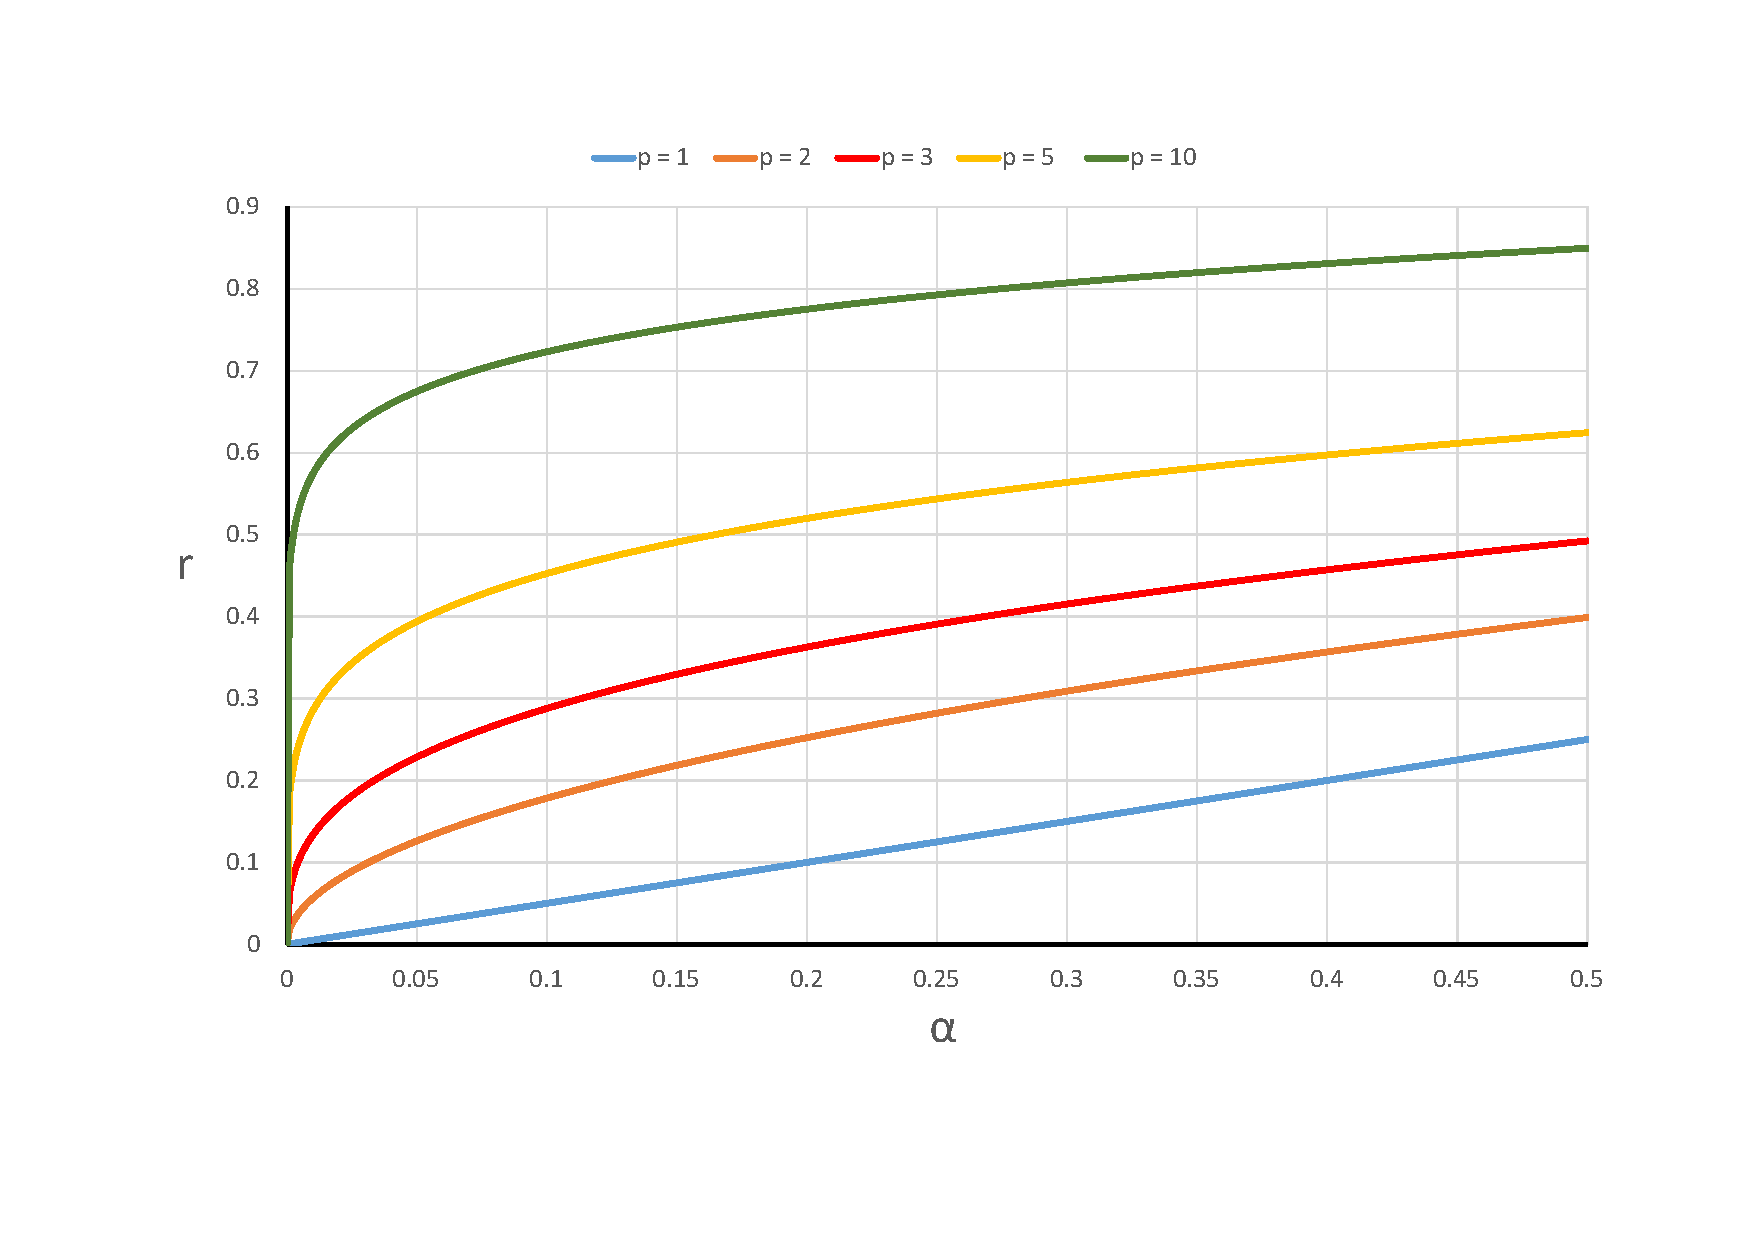
\includegraphics[width=0.7\linewidth]{images/supervised/knn_regression/radius.pdf}
	\end{center}

	\begin{itemize}
		\item con $\alpha=5$\% e $p=5$ abbiamo bisogno di un'ipersfera di raggio 0.4 in tutte le dimensioni
		\item e il problema peggiora al crescere di $p$
	\end{itemize}
\end{frame}
}

\begin{frame}

	\frametitle{Regressione k-NN, terza versione: caso classico con $\mathcal{N}_K(x)$}

	\begin{itemize}
		%\item La regressione k-NN è simile alla classificazione k-NN
		\item se definiamo, come solitamente viene fatto nel caso classico di k-NN, che $\mathcal{N}_K(x)$ contiene i $K$ elementi del dataset più vicini a $x$ nello spazio delle features
		\item quindi $\forall K, x$ vale che: $\sum_{i=1}^N \mathbb{I}[x_i\in\mathcal{N}_K(x)] = K$
		\item per prevedere $Y$ in corrispondenza di un certo $X$, consideriamo i $K$ punti più vicini a $X$ nel training set e calcoliamo la media dei valori della variabile di risposta:
			\[
				\widehat f(x) = \frac{\sum_{i=1}^N y_i \mathbb{I}[x_i\in\mathcal{N}_K(x)]}{\sum_{i=1}^N \mathbb{I}[x_i\in\mathcal{N}_K(x)]} = \frac{1}{K} \sum_{i=1}^N y_i \mathbb{I}[x_i\in\mathcal{N}_K(x)]
			\]
		\item se $K$ è piccolo, k-NN è molto più flessibile della regressione lineare
		\item ma siamo sicuri che questo sia sempre un vantaggio?
	\end{itemize}
\end{frame}



\subsubsection[L'accuratezza di un modello di regressione]{L'accuratezza di un modello di regressione}

\begin{frame}
	\frametitle{L'accuratezza di un modello di regressione}
	\begin{itemize}
		\item una \emph{misura di adattamento ai dati} è indispensabile per: 
			\begin{itemize}
				\item addestrare il modello (che sia parametrico o non parametrico)
				\item valutare il suo adattamento ai dati
			\end{itemize}
		\item supponiamo di stimare un modello di regressione $\widehat f(x)$ usando un certo campione, detto \emph{training set}, $\mathcal{TR}=\{(x_i,y_i),\,i=1,2,\ldots,n\}$
		\item l'\emph{Errore Quadratico Medio (di Previsione)} [\emph{Mean Squared (Prediction) Error}, (MSE)] over $\mathcal{TR}$:
			\[
				\mbox{MSE}_{\mathcal{TR}} = \frac{1}{n} \sum_{i=1}^n [y_i-\widehat f(x_i)]^2
			\]
		\item notare che $\widehat{f}(x)$ è selezionato \emph{minimizzando} $\mbox{MSE}_{\mathcal{TR}}$
	\end{itemize}
\end{frame}


\begin{frame}

	\frametitle{Regressione k-NN: l'accuratezza del modello}

	\begin{center}
		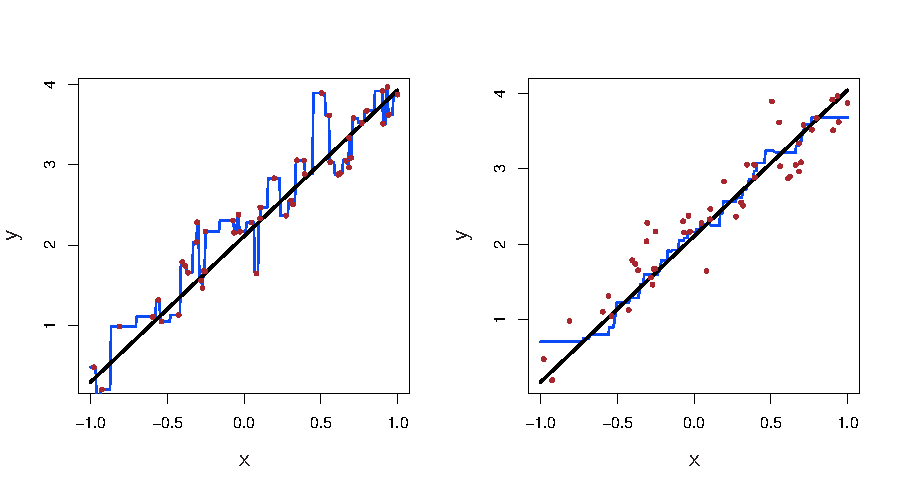
\includegraphics[scale=0.7]{images/supervised/knn_regression/3_17.pdf}\\
		Il vero modello che ha generato i dati è lineare.\\
		In blu viene mostrato il modello $\widehat{f}(x)$ stimato descritto da K-NN:\\
		a sinistra per $K=1$, a destra per $K=10$.
	\end{center}
\end{frame}


\begin{frame}

	\frametitle{L'accuratezza di un modello di regressione}

	\begin{itemize}
		\item come misura dell'adeguatezza di un modello, $\pmb{\mbox{MSE}_{\mathcal{TR}}}$ \textbf{è distorto a favore di modelli più flessibili}
		\item per misurare la performance di un modello dovremmo calcolare il MSE usando un \emph{test set}, osservazioni nuove non usate per addestrare il modello, $\mathcal{TE} = \{(\widetilde x_i,\widetilde y_i),\,i=1,2,\ldots,m\}$:
			\[
				\mbox{MSE}_{\mathcal{TE}} = \frac{1}{m}\sum_{i=1}^m [\widetilde y_i-\widehat f(\widetilde x_i)]^2
			\]
		\item in generale, il metodo con il $\mbox{MSE}_{\mathcal{TR}}$ più piccolo non è detto abbia il $\mbox{MSE}_{\mathcal{TE}}$ minimo
		\item studiamo più in profondità questo problema usando dati simulati, cercando di \textbf{approssimare} i dati con \textbf{polinomi di grado} $\pmb{n}$ (flessibilità)
	\end{itemize}
\end{frame}


\ifthenelse{\boolean{highschool}}{}{
\begin{frame}

	\frametitle{L'accuratezza di un modello di regressione: Esempio 1}

	\begin{itemize}
		\item a sinistra: la curva nera rappresenta la vera $f$
		\item a destra: la curva rossa rappresenta il MSE$_{\mathcal{TE}}$; quella grigia è il MSE$_{\mathcal{TR}}$; la curva tratteggiata è il minimo MSE$_{\mathcal{TE}}$ possibile -- l'errore irriducibile
		\item in entrambi i grafici: le curve e i punti arancio, blue e verde corrispondono a modelli con gradi di flessibilità diversi
	\end{itemize}

	\begin{figure}[!htbp]
		\centering
		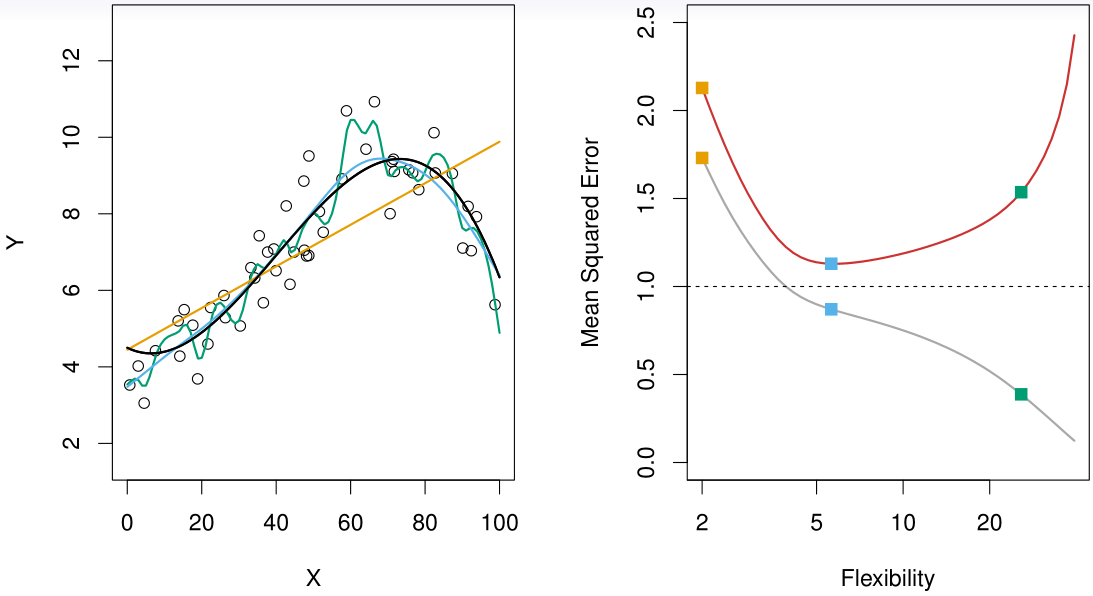
\includegraphics[width=0.6\linewidth]{images/supervised/knn_regression/g8.png}		%\caption{Stripe Radar for Fraud Detection}
	\end{figure}
\end{frame}

\begin{frame}

	\frametitle{L'accuratezza di un modello di regressione: Esempio 2}

	\begin{itemize}
		\item la legenda è la stessa dell'Esempio 1
		\item la vera $f$ è più regolare:
			\begin{itemize}
				\item I modelli meno flessibili si adattano molto bene
				\item MSE$_{\mathcal{TE}}$ e MSE$_{\mathcal{TR}}$ hanno la stessa forma generale del grafico precedente
			\end{itemize}
	\end{itemize}

	\begin{center}
		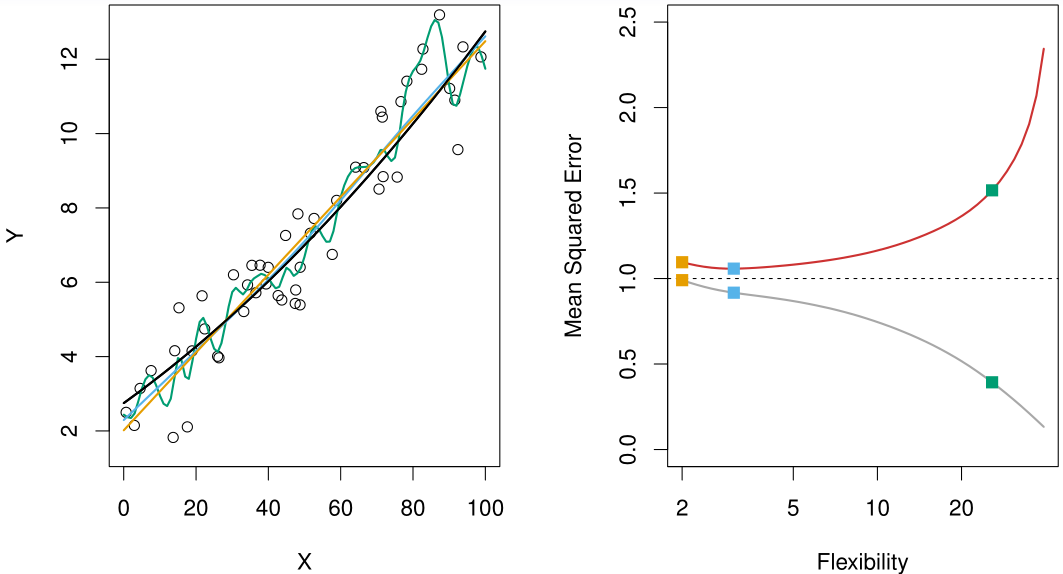
\includegraphics[scale=0.4]{images/supervised/knn_regression/g9.png}
	\end{center}

\end{frame}

\begin{frame}

	\frametitle{L'accuratezza di un modello di regressione: Esempio 3}

	\begin{itemize}
		\item la legenda è la stessa dell'Esempio 1
		\item la vera $f$ è più irregolare:
			\begin{itemize}
				\item I modelli più flessibili si adattano molto bene
				\item Di nuovo, MSE$_{\mathcal{TE}}$ e MSE$_{\mathcal{TR}}$ hanno lo stesso andamento generale
			\end{itemize}
	\end{itemize}

	\begin{center}
		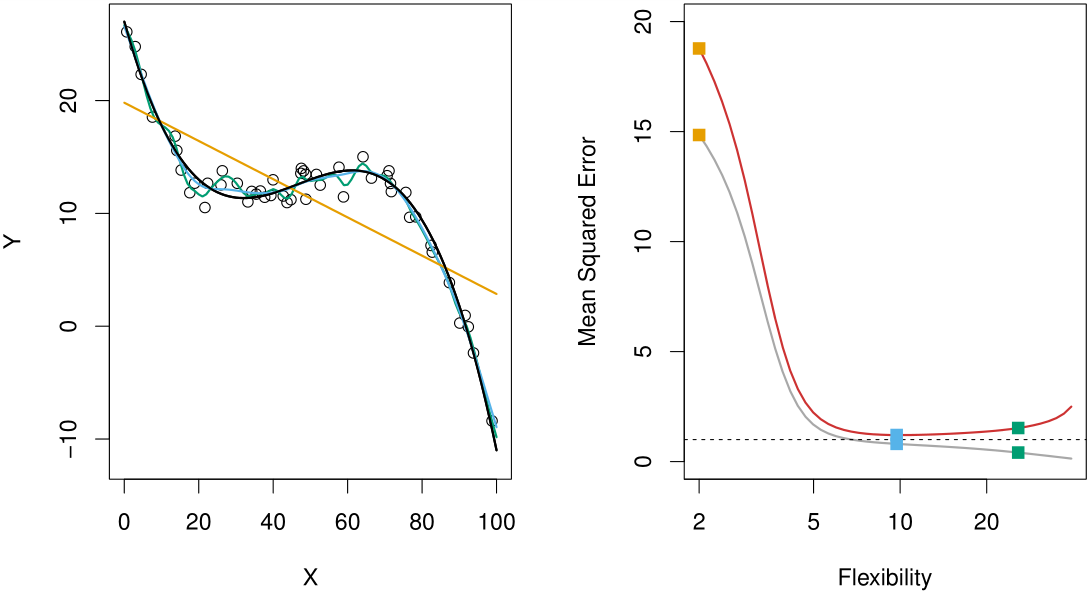
\includegraphics[scale=0.4]{images/supervised/knn_regression/g10.png}
	\end{center}

\end{frame}

}

\begin{frame}

	\frametitle{Un grafico fondamentale}

	\begin{center}
		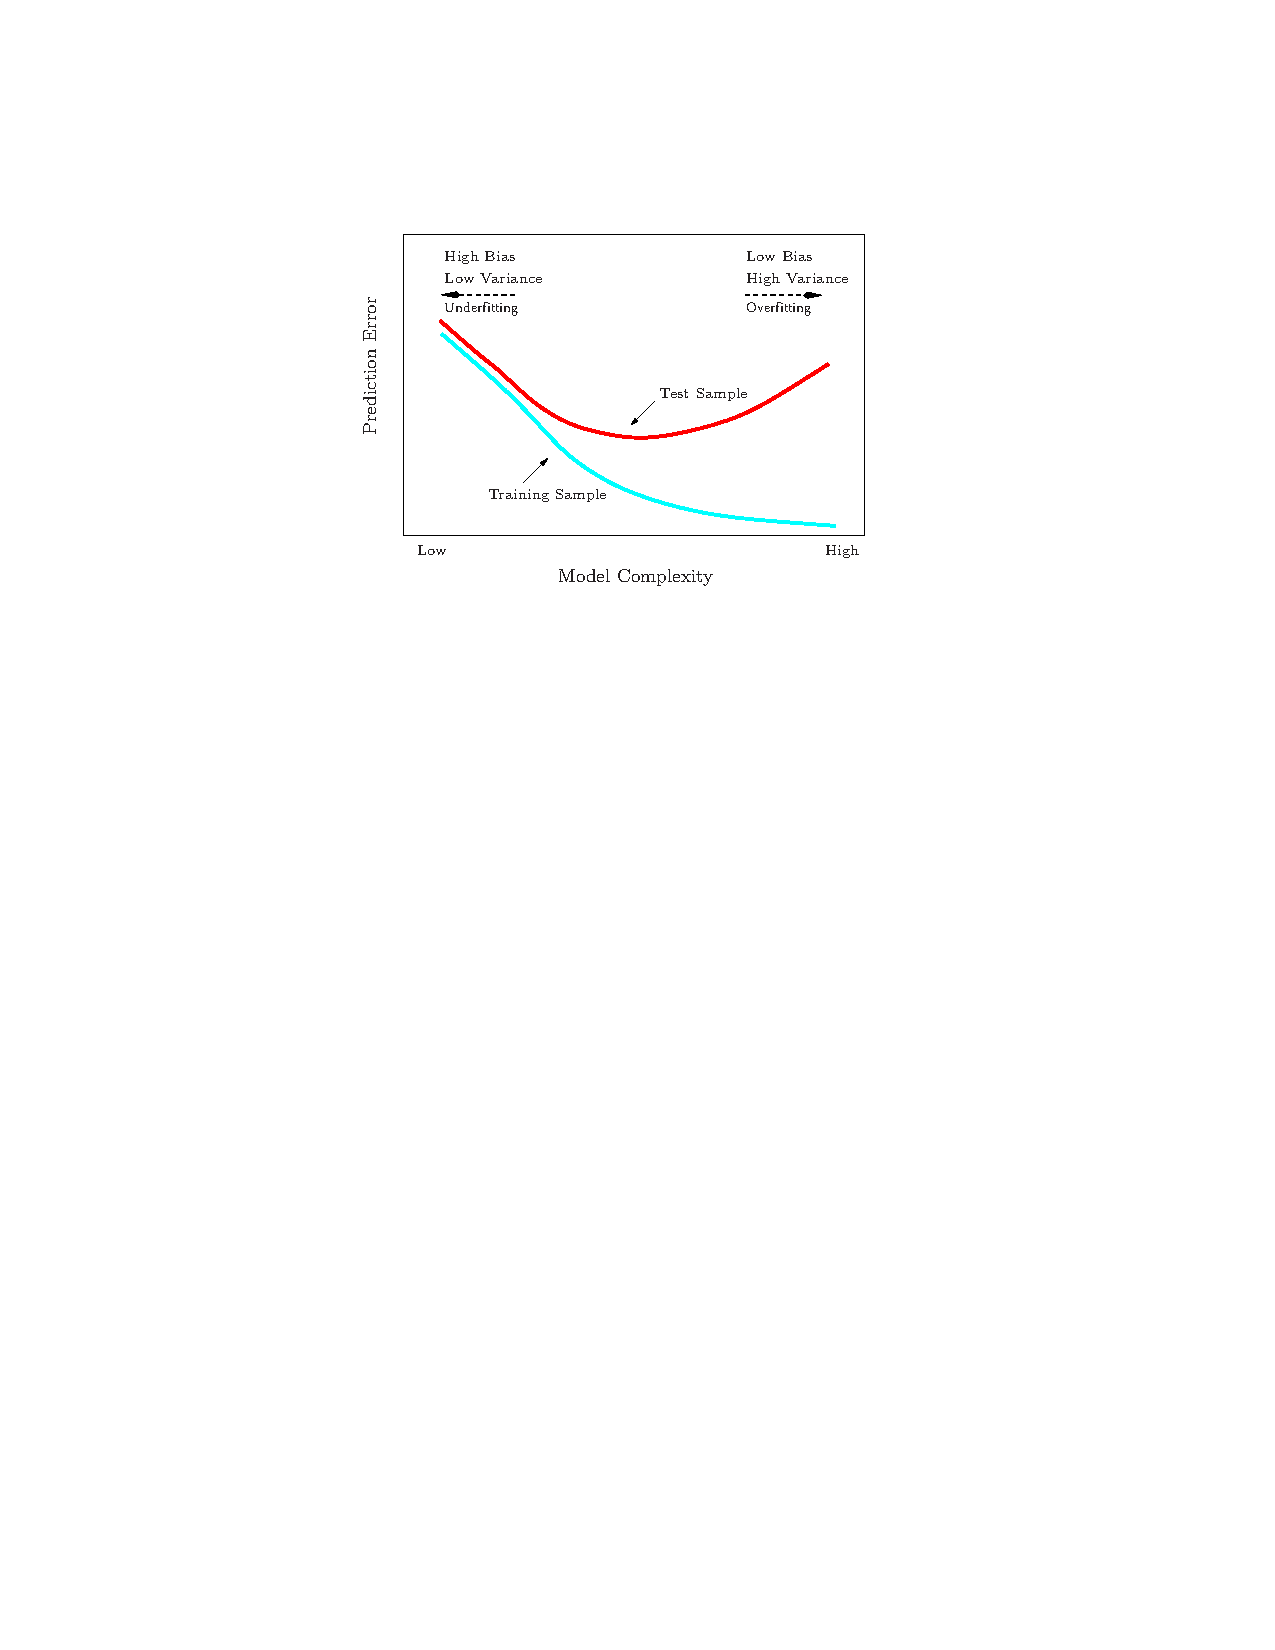
\includegraphics[scale=0.8]{images/supervised/knn_regression/MSE.pdf}
	\end{center}

	\begin{itemize}
		\item In generale:
			\begin{itemize}
				\item al crescere della flessibilità, il MSE$_{\mathcal{TR}}$ diminuisce sempre
				\item al crescere della flessibilità, il MSE$_{\mathcal{TE}}$ inizialmente diminuisce ma a un certo punto inizia a crescere
			\end{itemize}
	\end{itemize}
\end{frame}



\ifthenelse{\boolean{highschool}}{}{

\begin{frame}

	\frametitle{Regressione k-NN: l'accuratezza del modello}

	\begin{center}
		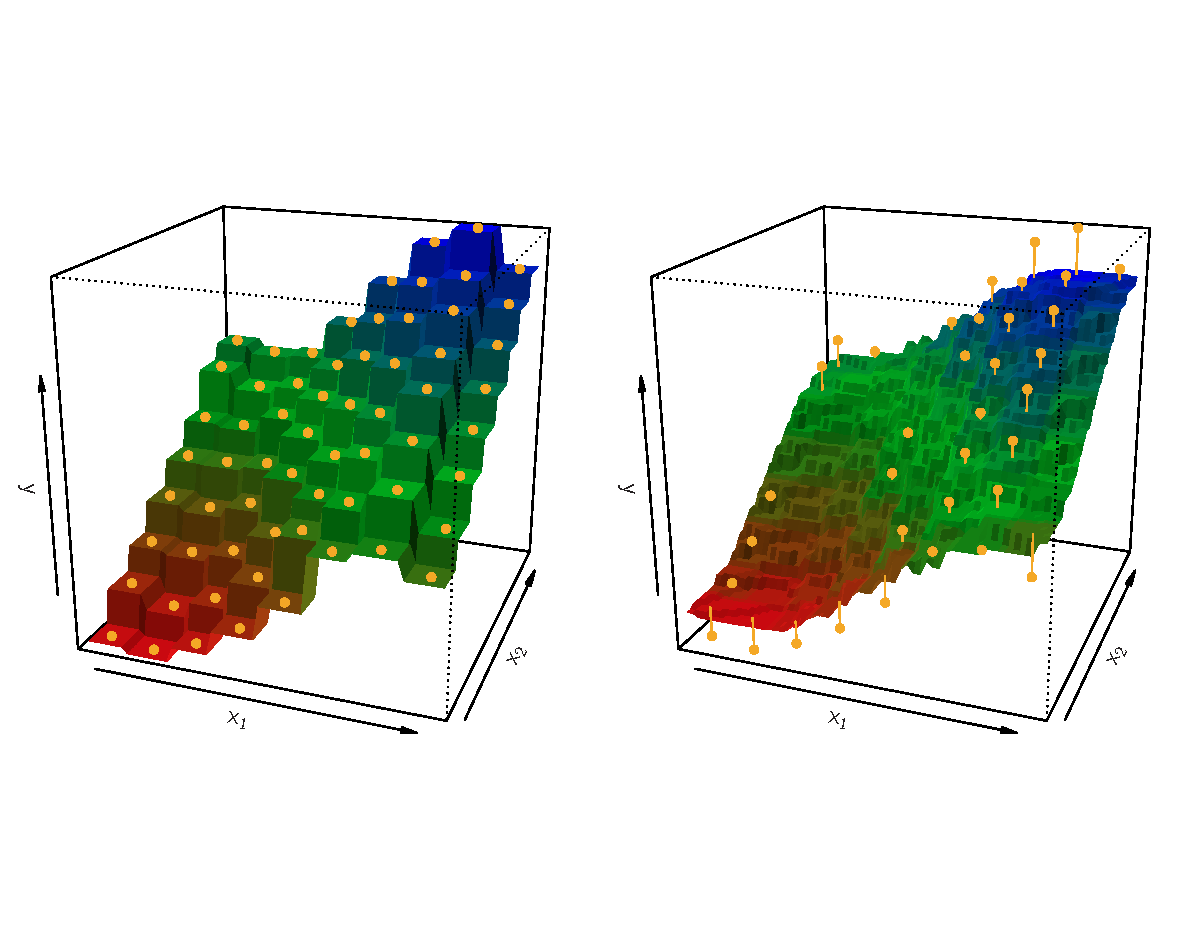
\includegraphics[width=1\linewidth]{images/supervised/knn_regression/3_16.pdf}\\
		Stime k-NN per $K=1$ e $K=9$\\(64 osservazioni simulate con $p = \dim(X)=2$)
	\end{center}
\end{frame}


\begin{frame}

	\frametitle{Regressione k-NN: l'accuratezza del modello}

	\begin{itemize}
		\item se il vero modello è lineare, k-NN funzionerà sempre peggio della regressione lineare
		\item più in generale: se indoviniamo la forma funzionale, un approccio parametrico sarà sempre superiore a uno non parametrico
	\end{itemize}

	\begin{center}
		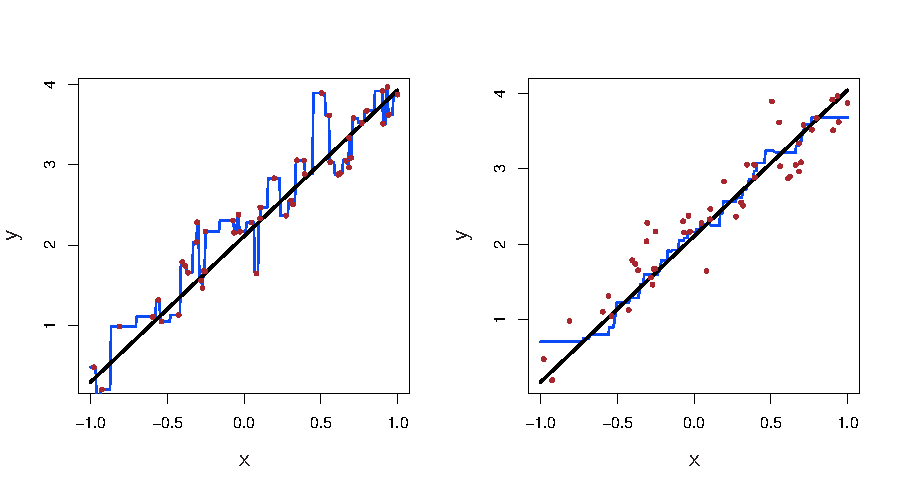
\includegraphics[scale=0.55]{images/supervised/knn_regression/3_17.pdf}\\
		Il vero modello è lineare (100 osservazioni simulate con $p = \dim(X)=1$)
	\end{center}
\end{frame}


\begin{frame}

	\frametitle{Regressione k-NN: l'accuratezza del modello}

	\begin{itemize}
		\item il MSE sul test set (a destra, in verde) della stima k-NN è sempre maggiore di quello della regressione lineare (a destra, tratteggiato)
	\end{itemize}

	\begin{center}
		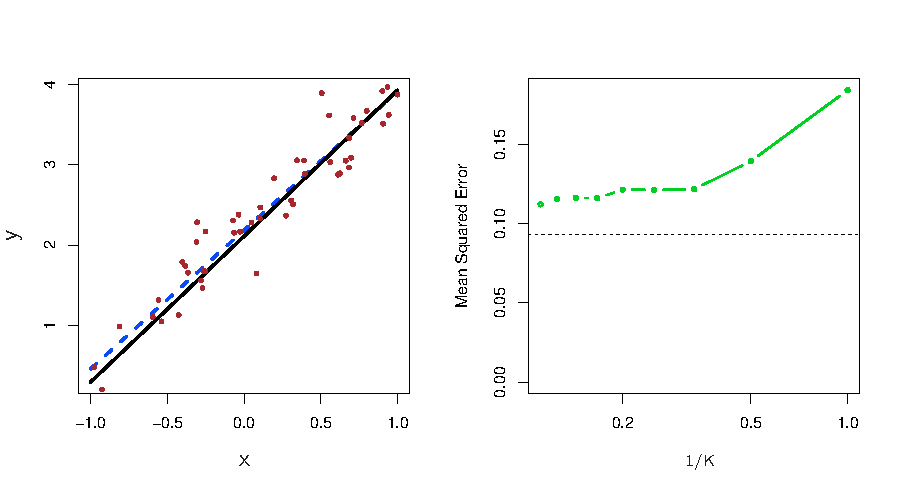
\includegraphics[scale=0.55]{images/supervised/knn_regression/3_18.pdf}\\
		Il vero modello è lineare (100 osservazioni simulate con $p = \dim(X)=1$)
	\end{center}
\end{frame}


\begin{frame}

	\frametitle{Regressione k-NN: l'accuratezza del modello}

	\begin{itemize}
		\item se la vera $f$ non è lineare, il predittore k-NN può essere migliore
	\end{itemize}

	\begin{center}
		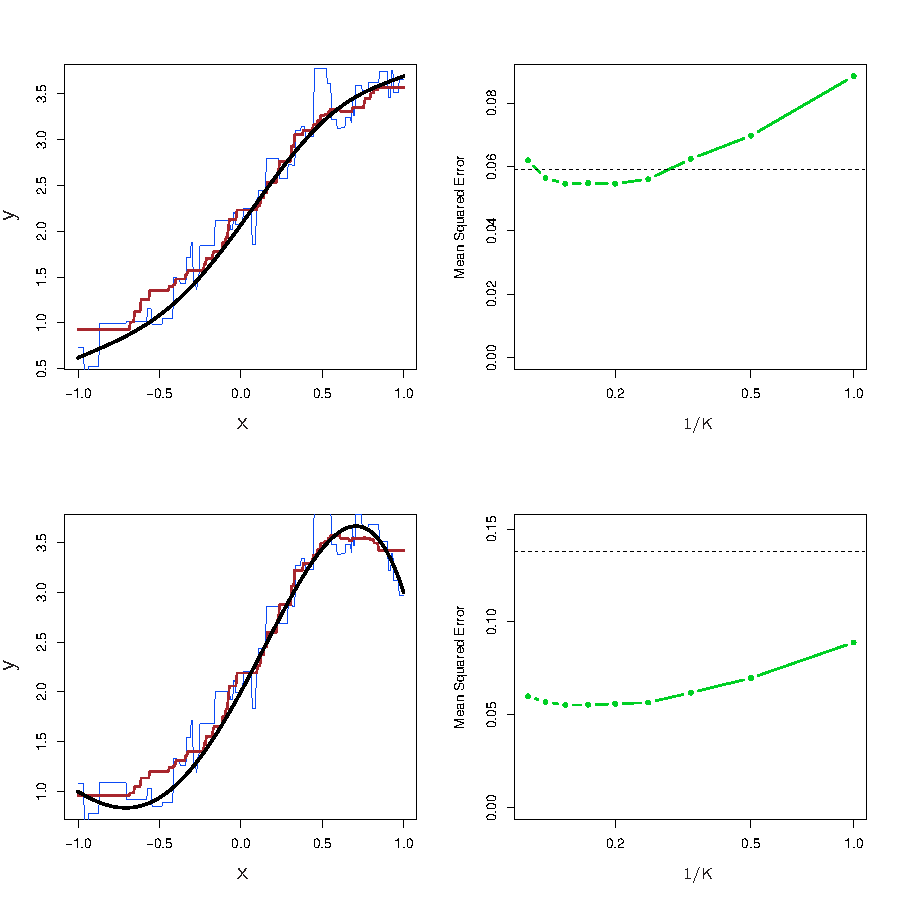
\includegraphics[scale=0.45]{images/supervised/knn_regression/3_19.pdf}\\
		Il vero modello è non lineare (100 osservazioni simulate con $p = \dim(X)=1$)
	\end{center}
\end{frame}


%\begin{frame}
%
%	\frametitle{Regressione k-NN: l'accuratezza del modello}
%
%	\begin{itemize}
%		\item anche con un vero modello non lineare, la performance del predittore k-NN peggiora al crescere di $p$ (maledizione della dimensionalità)
%	\end{itemize}
%
%	\begin{center}
%		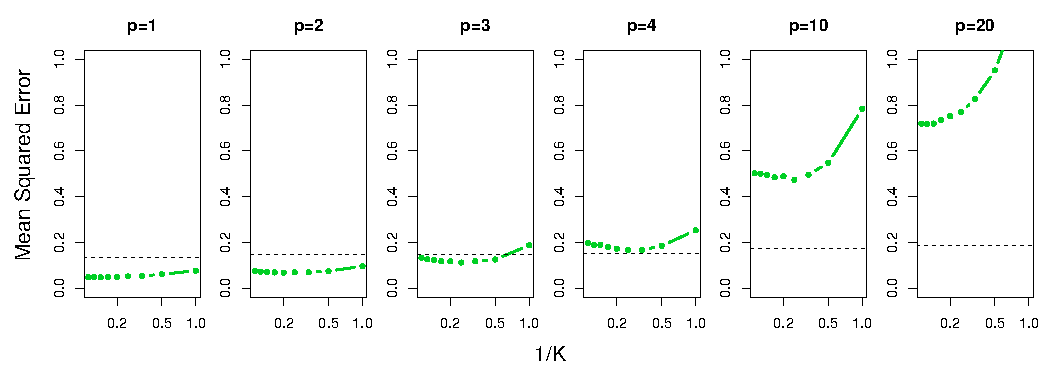
\includegraphics[scale=0.55]{images/supervised/knn_regression/3_20.pdf}\\
%		Il vero modello è non lineare\\(100 osservazioni simulate con $p = \dim(X)=1$;\\
%		le variabili $X$ di indice superiore o uguale a 2 contengono solo rumore)
%	\end{center}
%\end{frame}

}



\subsubsection[Classificazione k-NN]{\textit{Classificazione k-NN}}


\begin{frame}
	\frametitle{Problemi di classificazione, una formalizzazione}

	\begin{itemize}
		\item assumiamo che $Y$ sia qualitativa -- in altre parole, che assuma valori in un insieme discreto e finito $\mathcal{C}$
		\item vogliamo costruire un \emph{classificatore} $C(X)$ che assegni un'etichetta in $\mathcal{C}$ a un'osservazione $x_0$ che ne è priva
		\item possiamo usare il metodo k-NN esattamente come abbiamo fatto prima
			\begin{itemize}
				\item anche in questo caso funziona peggio al crescere di del numero di features (per via della \textit{maledizione della dimensionalità})
				%\item l'effetto su $\widehat{C}$ tuttavia è inferiore a quello su $\widehat p_k$
			\end{itemize}
	\end{itemize}

	\begin{center}
		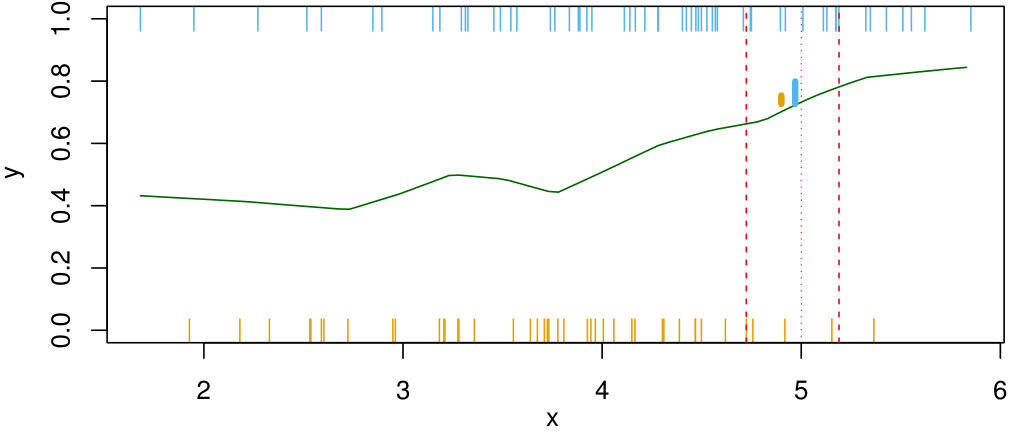
\includegraphics[width=0.7\linewidth]{images/supervised/knn_classification/knn_classification_r_plot.png}
	\end{center}
\end{frame}


\ifthenelse{\boolean{highschool}}{}{
\begin{frame}
	\frametitle{Problemi di classificazione, una formalizzazione}

	\begin{itemize}
		\item esiste un $C(X)$ ideale?
		\item supponiamo che gli elementi in $\mathcal{C}$ siano indicati da $1,2,...,J$. Definiamo le \emph{probabilità condizionali}:
			\[
				p_j(x) = \prob(Y=j|X=x), \quad j=1,2,\ldots,J
			\]
		\item il classificatore di \emph{Bayes} in $x$ è dato da
			\[
				C_{Bayes}(x) = h \quad \mbox{se} \quad p_h(x) = \max \{ p_1(x),p_2(x),\ldots,p_J(x)\}
			\]
		\item il classificatore di Bayes è \emph{ottimale} nel senso che minimizza la \emph{probabilità di errata classificazione nella popolazione}:
			\[
				C_{Bayes}(X) = \arg\min_C \prob[C(X)\not= Y]
			\]
			Questa proprietà vale \emph{nella popolazione} \emph{in corrispondenza delle vere $p_j$}
	\end{itemize}
\end{frame}
}



\begin{frame}

	\frametitle{Classificazione k-NN, esempio grafico con p = 2 (features)}

	\begin{columns}

		\column{0.5\linewidth}
		%Esempio di classificazione k-NN.
		Il campione di prova (punto verde) deve essere classificato in quadrati blu o in triangoli rossi.
		\begin{itemize}
			\item se k = 3 (cerchio a linea continua) viene assegnato ai triangoli rossi perché ci sono 2 triangoli e solo 1 quadrato all'interno del cerchio interno
			\item se k = 5 (cerchio linea tratteggiata) viene assegnato ai quadrati blu (3 quadrati contro 2 triangoli all'interno del cerchio esterno)
		\end{itemize}


		\column{0.5\linewidth}
		\begin{figure}[!htbp]
			\centering
			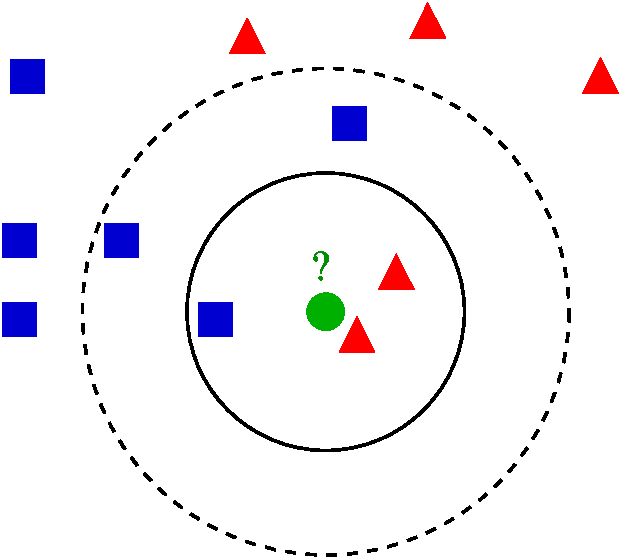
\includegraphics[width=0.75\linewidth]{images/supervised/knn_classification/knn_classification_radius.pdf}
			%\caption{Complete-Link}
			%\label{Enel_QQ_Plot_Normal}
		\end{figure}

	\end{columns}

\end{frame}

\ifthenelse{\boolean{highschool}}{}{
\begin{frame}
	\frametitle{Classificazione k-NN, esempio grafico 2}
	\begin{center}
		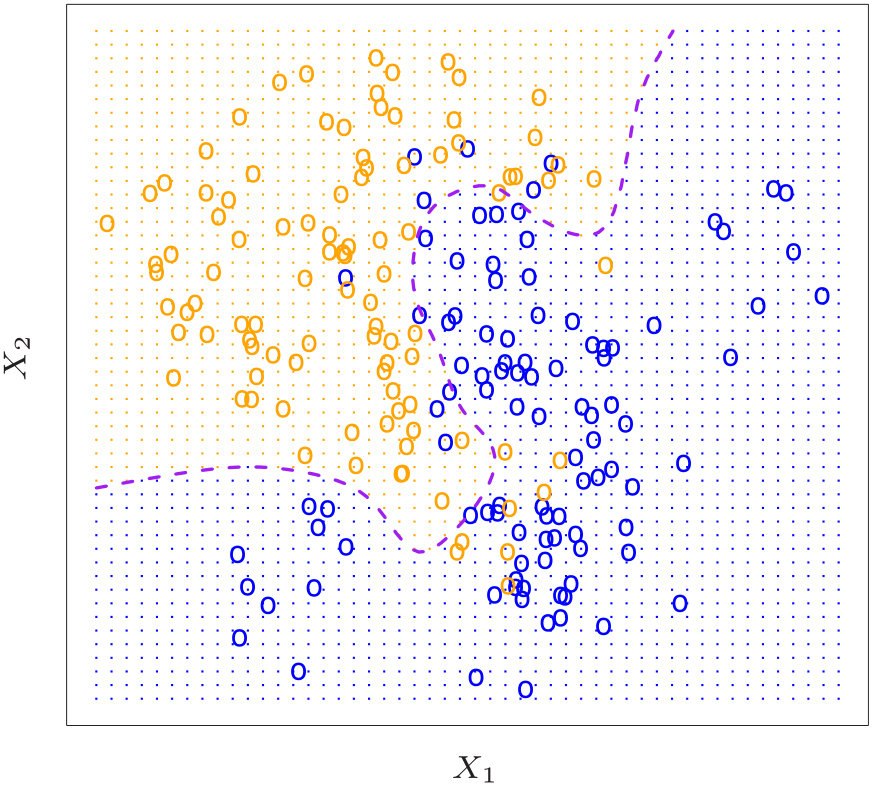
\includegraphics[width=0.5\linewidth]{images/supervised/knn_classification/knn_classification_example_1.png} \\ Bayes classifier
	\end{center}
\end{frame}
}


\subsubsection[L'accuratezza di un modello di classificazione]{L'accuratezza di un modello di classificazione}
\begin{frame}
	\frametitle{L'accuratezza di un modello di classificazione}

	\begin{itemize}
		\item di solito misuriamo la performance di $\hat C$ usando il tasso di errata classificazione su un test set:
			\begin{empheq}[box=\fcolorbox{blue!40!black!60}{yellow!10}]{align*}
			\mbox{Err}_{\mathcal{TE}} = \frac{1}{n} \sum_{i=1}^n \mathbb{I}[\widetilde y_i\not= \hat C(\widetilde x_i)]
			\end{empheq}
%			\makebox[\textwidth]{$\mbox{Err}_{\mathcal{TE}} = \frac{1}{n} \sum_{i=1}^m \mathbb{I}[\widetilde y_i\not= \hat C(\widetilde x_i)]$}
		\item $\mbox{Err}_{\mathcal{TE}}$: stima probabilità di errata classificazione nella popolazione
		\item nella popolazione, nessun classificatore può raggiungere tassi d'errore inferiori a quelli del classificatore di Bayes (il tasso d'errore del classificatore di Bayes è l'errore irriducibile)
		\item in pratica, il classificatore di Bayes \emph{non può essere calcolato} -- non conosciamo le \emph{vere} probabilità $p_j$
		\item possiamo imitarlo usando probabilità \emph{stimate} $\widehat p_j$
		\item in un esempio basato su osservazioni simulate con $p=2$ e $J=2$, il classificatore k-NN assegna a ogni $x_0=(x_{01},x_{02})^\prime$ l'etichetta con il maggior numero di osservazioni nell'intorno
	\end{itemize}
\end{frame}


\begin{frame}
	\frametitle{Classificazione k-NN, esempio grafico 2}
	\begin{center}
		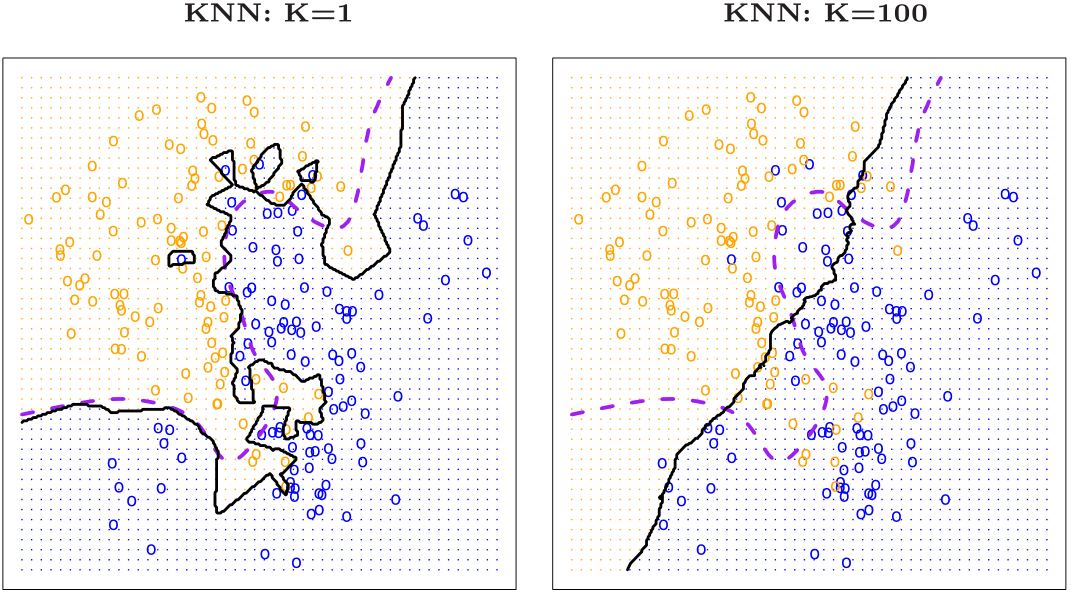
\includegraphics[width=1.0\linewidth]{images/supervised/knn_classification/knn_classification_example_3.png}
	\end{center}
\end{frame}


\begin{frame}
	\frametitle{Classificazione k-NN, esempio grafico 2}

	\begin{center}
		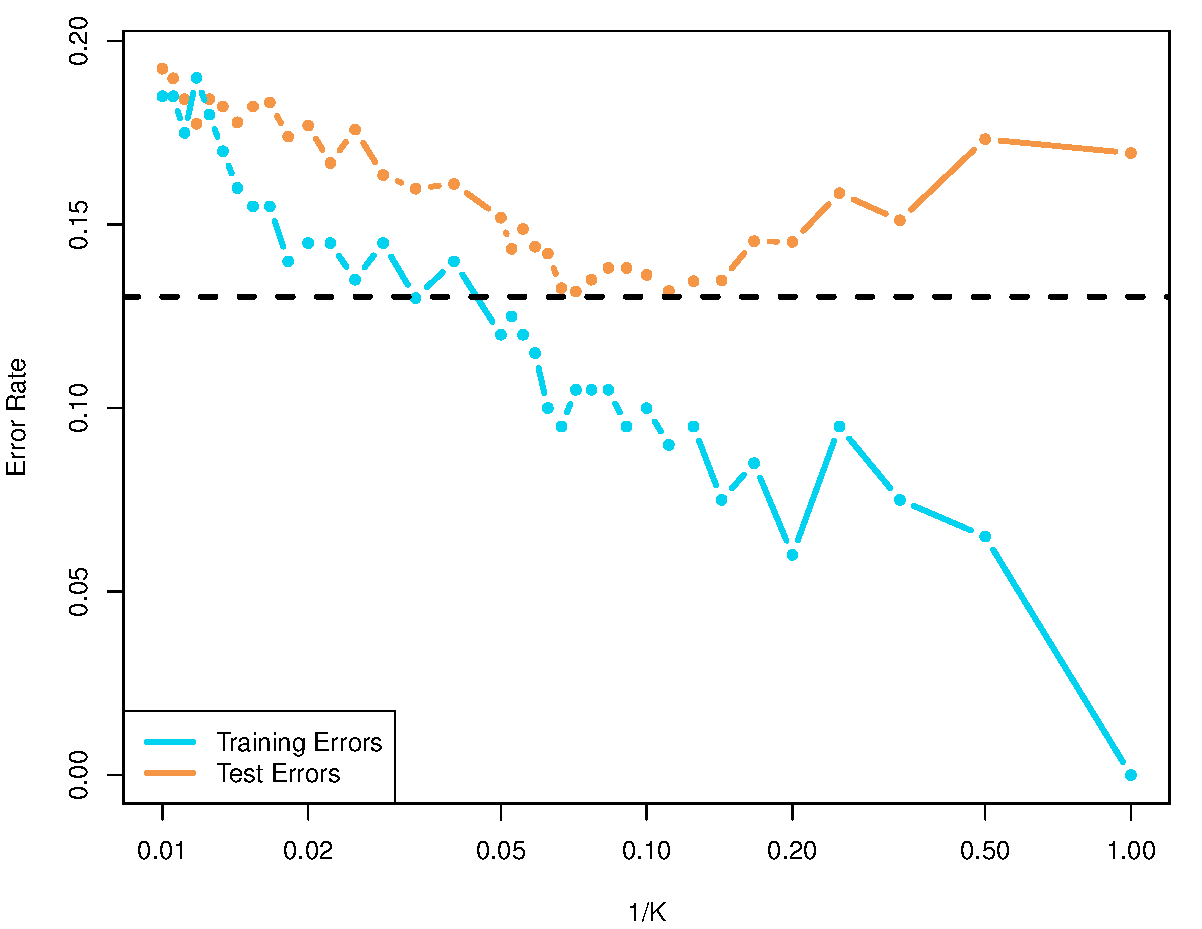
\includegraphics[scale=0.4]{images/supervised/knn_classification/2_17.pdf}
	\end{center}

	\begin{itemize}
		\item L'andamento dei tassi di errore nel training e nel test set è lo stesso visto prima!
	\end{itemize}
\end{frame}

\begin{frame}
	\frametitle{Classificazione k-NN, esempio grafico 2}
	\begin{center}
		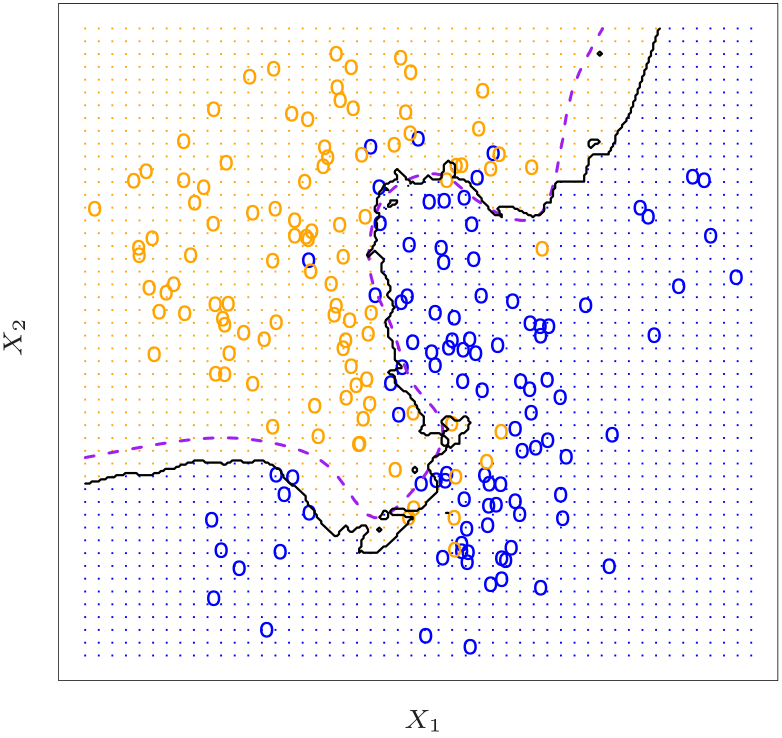
\includegraphics[width=0.5\linewidth]{images/supervised/knn_classification/knn_classification_example_2.png} \\ $K=10$
	\end{center}
\end{frame}

